% comment
%%%%%%%%%%%%%%%%%%%%%%% file typeinst.tex %%%%%%%%%%%%%%%%%%%%%%%%%
%
% This is the LaTeX source for the instructions to authors using
% the LaTeX document class 'llncs.cls' for contributions to
% the Lecture Notes in Computer Sciences series.
% http://www.springer.com/lncs       Springer Heidelberg 2006/05/04
%
% It may be used as a template for your own input - copy it
% to a new file with a new name and use it as the basis
% for your article.
%
% NB: the document class 'llncs' has its own and detailed documentation, see
% ftp://ftp.springer.de/data/pubftp/pub/tex/latex/llncs/latex2e/llncsdoc.pdf
%
%%%%%%%%%%%%%%%%%%%%%%%%%%%%%%%%%%%%%%%%%%%%%%%%%%%%%%%%%%%%%%%%%%%


\documentclass[letter]{llncs}

\usepackage{amssymb}
\setcounter{tocdepth}{3}
\usepackage{graphicx}
\usepackage{amsmath}
% \usepackage[options]{algorithm2e}
% \usepackage{algorithm}% http://ctan.org/pkg/algorithms
\usepackage{algpseudocode}% http://ctan.org/pkg/algorithmicx
\usepackage{algorithm}

\makeatletter
\renewcommand{\ALG@beginalgorithmic}{\small}
\algrenewcommand\algorithmicindent{0.5em}%
\makeatother
\usepackage[caption=false,font=footnotesize]{subfig}
\usepackage{url}
\urldef{\mailsa}\path|{alfred.hofmann, ursula.barth, ingrid.haas,
frank.holzwarth,|
\urldef{\mailsb}\path|anna.kramer, leonie.kunz, christine.reiss, nicole.sator,|
\urldef{\mailsc}\path|erika.siebert-cole, peter.strasser, lncs}@springer.com|  
\usepackage{listings}
\usepackage{enumerate}
\usepackage{textcomp}
\DeclareMathSizes{10}{10}{9}{9}
\usepackage{algpseudocode}% http://ctan.org/pkg/algorithmicx

\begin{document}
% New definitions
\algnewcommand\algorithmicswitch{\textbf{switch}}
\algnewcommand\algorithmiccase{\textbf{case}}
\algnewcommand\algorithmicassert{\texttt{assert}}
\algnewcommand\Assert[1]{\State \algorithmicassert(#1)}%

% New "environments"
\algdef{SE}[SWITCH]{Switch}{EndSwitch}[1]{\algorithmicswitch\ #1\ \algorithmicdo}{\algorithmicend\ \algorithmicswitch}%
\algdef{SE}[CASE]{Case}{EndCase}[1]{\algorithmiccase\ #1}{\algorithmicend\ \algorithmiccase}%
\algtext*{EndSwitch}%
\algtext*{EndCase}%
% first the title is needed
\title{From UML to Process Algebra and Back:\\An Automated Approach to
Model-Checking Software Design Artifacts of Concurrent Systems}

% a short form should be given in case it is too long for the running head

% the name(s) of the author(s) follow(s) next
%
% NB: Chinese authors should write their first names(s) in front of
% their surnames. This ensures that the names appear correctly in
% the running heads and the author index.
%
\author{Daniela Remenska\inst{1,3}
\and Jeff Templon\inst{3} \and Tim A.C. Willemse\inst{2} \and Philip Homburg\inst{1} \and\
Kees Verstoep\inst{1} \and Adria Casajus\inst{4} \and Henri Bal\inst{1}}
%
% (feature abused for this document to repeat the title also on left hand pages)

% the affiliations are given next; don't give your e-mail address
% unless you accept that it will be published
\institute{Dept. of Computer Science, VU University Amsterdam, The Netherlands
\and
Dept. of Computer Science, TU Eindhoven, The Netherlands
\and
NIKHEF, Amsterdam, The Netherlands
\and
Universitat de Barcelona, Spain
}
%
% NB: a more complex sample for affiliations and the mapping to the
% corresponding authors can be found in the file "llncs.dem"
% (search for the string "\mainmatter" where a contribution starts).
% "llncs.dem" accompanies the document class "llncs.cls".
%

\toctitle{Lecture Notes in Computer Science}
\tocauthor{Authors' Instructions}
\maketitle
\vspace{-15 pt}
\begin{abstract}
One of the challenges in software development is early discovery of design
errors which could lead to deadlocks or race-conditions. For safety-critical and
complex distributed applications, traditional testing does not always expose such
problems, so abstract models are necessary for performing formal
analysis. For object-oriented software, UML is the industry-adopted modeling
language. UML offers a number of views to present the system from different
perspectives. Behavioral views are necessary for the purpose of model checking,
as they capture the dynamics of the system. Among them are sequence diagrams, in
which the interaction between components is modeled by means of message
exchanges. UML 2.x includes rich features that
enable modeling code-like structures, such as loops, conditions and refering to
existing interactions.
We present an automatic procedure for translating UML into mCRL2 process algebra
models. Our prototype is able to
produce a formal model, and feed model-checking traces back into any
UML modeling tool, without the user having to leave the UML domain. We argue why
previous approaches of which we are aware have limitations that we overcome. We
further apply our methodology on the Grid framework used to support production
activities of one of the LHC experiments at CERN.
\keywords{formal methods, software engineering, UML}
\end{abstract}

\section{Introduction}
\label{sec:Introduction}
As modern software systems become more complex and distributed, a major
challenge is faced 
in maintaining their quality and functional correctness. Early discovery of
design errors which could
lead to deadlocks, race-conditions and other flaws, before they can surface,
is of a paramount importance.
The Unified Modeling Language (UML) \cite{UML2.4} has become the lingua franca
of software engineering, in particular for the domain of object-oriented
systems. Over time, several mature CASE tools have already adopted UML as the
industry-standard visual modeling language for describing software systems. 
However, use of these tools alone does not
assure the correctness of the design, nor does it provide direct means to test
the software under design,
let alone prove certain properties of interest, such as the absence of deadlocks. 
For safety-critical and complex
distributed applications, traditional testing of the resulting software tends 
to not always expose
such problems, so abstract models are necessary for formal analysis.  
In the last decades, more rigorous methods and tools for modeling and analysis
 have been proposed. Despite the research effort,
these methods are still not widely
accepted in industry. One problem is the lack of expertise and the necessary
time investment in the OO development cycle, for becoming proficient in them. 
A more substantial problem is the lack of a systematic connection between 
actual implementation and the semantics of the existing formal languages. 

To bridge the gap between industry-adopted methodologies based on UML
software designs, and the sophisticated analysis, verification and optimization tools, several approaches have been proposed for
automated extraction of the necessary analysis models from the UML artifacts. For instance, Petri
Nets \cite{DBLP:journals/tse/DistefanoSP11,Bernardi:2002:USD:584369.584376}, Layered 
Queuing Networks \cite{Petriu:2002:AUP:647810.737982}
and stochastic process algebras
\cite{Tribastone:2008:AEP:1383559.1383569,Tribastone:2008:ATU:1446304.1447447} are used for performance
analysis. Model checking for certain properties of the system is often done via
translation into process algebra
\cite{10.1109/APSEC.2005.7,inpJuDuJuLaPo06a}. Automatic synthesis of functional
test cases from UML models is possible as well
\cite{Bandyopadhyay:2009:TIG:1547558.1548197,Pickin02systemtest,Dinh-Trong:2006:SAG:1190616.1191226}. 
Model-to-model transformations
can also be done within the UML domain itself, for the purpose of model optimization or
refactoring \cite{Whittle:2002:TSM:647246.719610}.
In each of these cases, the translation is mediated by defining
graph-transformation rules between the meta models of UML and the target language.
\vspace{-1 pt}

A UML model of a system is typically a combination of multiple views. 
Devising an automated transformation
methodology 
requires that behavioral views of the system be available. The static views of
a system (such as Class and Deployment UML diagrams) are rarely sufficient to
extract the necessary information for constructing a target model for meaningful analysis. 
Activity, Sequence, and State Machines are among the most commonly used behavioral diagrams
for this purpose.
State Machines (SM) represent the reaction of individual objects on different stimuli;
they are suitable for describing 
specific parts of systems, such as a critical control component, but are very
rarely used \cite{inpJuDuJuLaPo06a} as the sole paradigm for developing large
distributed object-oriented systems. Developers almost never
create a fully-formed object a-priori and in isolation, with all the behavior that the object will ever
need.
On the other hand, Activity Diagrams (AD) describe the system at a higher level of
abstraction, where objects and message exchanges are not captured. They represent 
workflows of activities, with support for choice and concurrency, and 
are commonly used for business process modeling. 
Sequence Diagrams (SD) provide the most fine-grained runtime view of
the system. 
They model a set of interacting objects by means of message-exchanges over time.
These diagrams contain information about the control flow during the
interaction, capturing 
conditions and iterations. With the introduction of UML 2.x set of rich features
such as combined fragments, SDs have become popular for expressing scenarios because of their clear
and intuitive visual layout and close correspondence with actual code-like
structures. However,
most of the proposed transformation approaches up to date target only one
particular type of
behavioral diagram, mostly AD or SM diagrams
\cite{Tribastone:2008:AEP:1383559.1383569,inpJuDuJuLaPo06a,Cao:2006:TMV:1169227.1169783,E_business,Siveroni:2008:PSS:1371602.1371879}. When it comes
to
interactions (SDs) or targeting multiple diagram types, the existing approaches either deal with UML 1.x
semantics \cite{Tribastone:2008:ATU:1446304.1447447,sarma1,Rasch:2005:CVS:2144745.2144752,GallardoMP02,pokozy-korenblat_04_toward}, 
largely limiting the expressiveness by not taking into account
all
elements which allow designers to describe complex traces in compact manner, 
or their semantical models suffer from flaws
\cite{Tribastone:2008:ATU:1446304.1447447,pokozy-korenblat_04_toward}, as we will show.
Furthermore, rarely \cite{Hansen:2010:AVE:2188418.2188435} does an approach give feedback to the software developer 
on the results of the formal analysis, back into the UML domain. 

Our interest in this paper is obtaining a formal model in the Algebra of
Communicating Processes (ACP \cite{process_algebra}) process algebra mCRL2
\cite{FormalLanguagemCRL2},
taking a UML model as starting point. We chose mCRL2 because it is able to deal
with abstract
data types as well as user-defined functions for data transformation.
Familiarity with the toolset's simulation,
debugging,
visualization and model-checking capabilities has
influenced our decision, although in principle, ACP has many commonalities with
other process algebraic formalisms,
so the methodology can be easily adapted.
The proposed approach in this paper is based on UML 2.x semantics, and makes use
of both sequence and activity diagrams to automatically derive the target formal model.
We rely on the XMI representation
to devise the model transformation procedure. XMI \cite{UML2.4} is an XML-based vendor-independent format for metadata exchange between
compliant UML tools.
Based on the approach, we have
developed 
a prototype tool that can take a UML model in XMI representation as input, and
construct
the mCRL2 model. Our methodology allows traces from the model
checking tool 
to be conveniently displayed back in any UML tool. 
We have further applied the tool to the DIRAC \cite{DIRAC_CommGridSolution} Grid
framework used to support production activities
for one of the LHC experiments.

The paper is structured as follows: Section~\ref{sec:Preliminaries} gives a brief overview of the 
syntax and semantics of the UML and mCRL2 language notation necessary for understanding the Transformation Methodology (Section~\ref{sec:Methodology}).
In Section~\ref{sec:Application} we apply it on a case study from the Grid domain, and we conclude in Section~\ref{sec:Conclusions}.
\vspace{-7 pt}
\section{Preliminaries}
\label{sec:Preliminaries}
\vspace{-7 pt}
The UML abstract syntax and semantics is described in terms of its \emph{UML metamodel},
which defines the relationships between model elements.
To translate a system composed of different diagrams, we chose Sequence 
Diagrams as a driving behavior description type, and we take the necessary additional information about concurrency
from Activity Diagrams. Our choice is motivated by the fact that SDs provide the richest set of constructs 
for low-level behavior expression, and as such have a close correspondence with actual code. 
Additional information from ADs is necessary for deriving the actual (OS level) processes,
relevant for concurrent and distributed systems. 
\vspace{-10 pt}
\subsection{Sequence Diagrams}
\label{sec:SDs}
\vspace{-2 pt}
Sequence diagrams model the interaction among a set of participants, with emphasis on the sequence of messages exchanged over time. 
The participants are class instances (objects) shown as rectangular boxes, with the vertical lines falling from them
known as \emph{Lifelines} (See Fig.~\ref{fig:example1}). 
\vspace{-1 pt}
\begin{figure}
\centering
\vspace{-20 pt}	
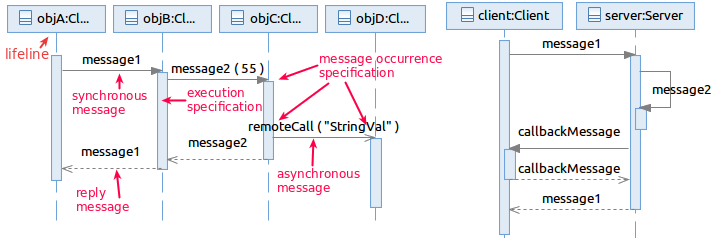
\includegraphics[width=1.0\linewidth,keepaspectratio=true]{./Figure1_new.png}
\caption{Sequence Diagrams notation}
\label{fig:example1}
\end{figure}
\vspace{-10 pt}
Each \emph{Message} sent between the lifelines defines a specific act of communication, synchronous or asynchronous. 
The start and end of the directed edge representing a message are called \emph{MessageEnds}, and are marked with 
a so called \emph{MessageOccurrenceSpecification} element of the UML metamodel, i.e., the 
occurrence of the send or receive event on the sender's and receiver's lifeline respectively.
Synchronous messages are drawn with filled arrow-head, while asynchronous ones have an open arrow-head.
Reply messages are drawn as dashed lines. All message types can carry zero or more arguments.

Messages are sent between objects with the aim of invoking specific behavior, known as
\emph{ExecutionSpecification}, and visualized as a thin rectangle on the receiver's lifeline. Thus,
execution specifications specify when a particular object is busy executing the invoked method.
Execution specifications can be nested/overlapping, as a result of a callback message, or 
an object invoking its own method, an example of both shown in Fig.~\ref{fig:example1} (right).
In this example,
the \emph{client} object sends a request for \emph{message1} execution on the \emph{server} side, after which 
it is blocked until it receives a reply from that method call. However, this does not stop other potential objects
from invoking any method of the \emph{client} interface. This possibility of overlapping method executions
on the lifeline on a single object plays an important role in our transformation methodology choices, as will become clear later. 
\vspace{-14 pt}
\subsubsection{Combined Fragments}
\label{sec:CombinedFragments}
Combined Fragments were introduced to add more expressiveness to SDs by 
means of constructs capturing complex control flows, thus overcoming many limitations 
present in UML 1.x. The specification supports different fragment types,
such as \emph{alt}, \emph{opt}, \emph{loop}, \emph{break}, \emph{par}.
They are visualized as rectangles with a keyword in the top-left corner indicating the type.
Combined Fragments consist of one or more \emph{InteractionOperands}. Depending on the type
of the fragment, \emph{InteractionConstraints} can guard each of the interaction operands.
Combined fragments can be nested with an arbitrary nesting depth, to capture complex workflows. Figure~\ref{fig:example3}
% \vspace{-13 pt}
\begin{figure}
\centering
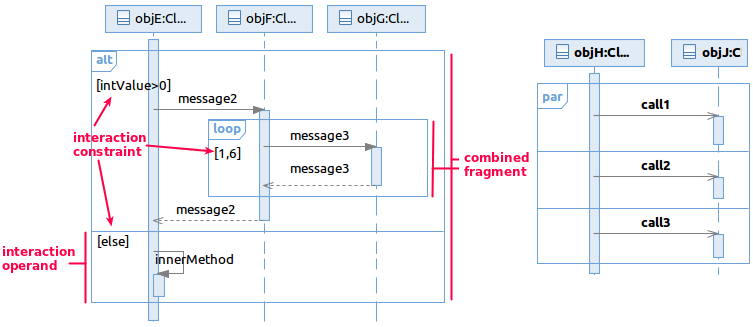
\includegraphics[width=1.0\linewidth,keepaspectratio=true]{./Figure2_merged.png}
\caption{Combined Fragments example}
\label{fig:example3}
\end{figure}
% \vspace{-13 pt}
shows how some of them can be used. The guards play a crucial role in deciding which fragment's operand(s) will
be executed at runtime. For more information on the semantics of combined fragments, the reader can refer to \cite{UML2.4}.

All fragment types above have equivalent constructs in most object oriented languages. 
Another useful enhancement is the \emph{InteractionUse} fragment. For expressing
complex scenarios, one can include a reference to another SD, which is semantically
equivalent to including the behavior of the called diagram in the current one. This promotes reuse of already defined
sequence diagrams. 
\vspace{-14 pt}
\subsubsection{Runtime Semantics}
Unlike the syntax, the SD semantics is scattered through the UML specification, and defined by the means of natural language. 
The most important points can be summarized as follows: the sending of a message is caused by previous message
receptions, and is the object's reaction to these receptions. In that sense, an object does not control the reception of a message.
Message and execution completion are considered local concepts.
For a message \emph{m} sent from object \emph{o1} to object \emph{o2}, the sender's view of that message completion is 
the sending, the receiver's view of the message completion is its reception, while other objects have no knowledge of \emph{m}.
Thus, the only synchronization points between the objects are the message exchanges.
\emph{This semantics does not impose a total ordering of the messages in a given SD.}
\vspace{-10 pt}
\subsection{Activity Diagrams}
As already stated, we use ADs to extract concurrency information necessary for deriving OS-level processes
in a distributed system setup. Although the notion of concurrency is present in some form in SDs, 
the \emph{par} fragment only indicates
that the implementation can execute any interleaving of the operands' behaviors, without mandating that the implementation be concurrent or distributed. 
In a concurrent or distributed setup, each of the SDs could be parts of multiple processes that must be initialized by
the system environment at some point, and this is where elements of ADs help.
We defer the explanation of the limited subset of used elements to the section where we explain the 
transformation methodology, illustrating it on an example.
% We give here only a limited subset of the concrete syntax necessary for our transformation methodology.
% 
% An example of a workflow modeled with this diagram type is illustrated in Fig.~\ref{fig:activity}.
% It consists of \emph{Action} and \emph{Control Nodes} connected by \emph{Activity Edges}, with each diagram having one distinguished \emph{Initial Node}. 
% The control flow nodes have their intuitive meaning as in traditional flow charts, namely to depict 
% concurrent flows (\emph{Fork}), their eventual join or synchronization (\emph{Join}), and decision points (\emph{Decision}).
% While there are various action types, we are primarily interested in the \emph{CallBehaviorAction}, which
% invokes a referenced behavior directly. Since SDs are also classified as behavior, we use this action type
% to provide the link between SDs and the concurrent system setup described in an AD.
% \begin{figure}
% \centering
% 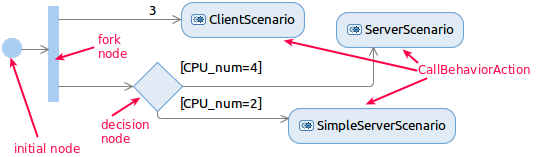
\includegraphics[width=0.8\linewidth,keepaspectratio=true]{./Figure3_new.png}
% \caption{Activity Diagram example}
% \label{fig:activity}
% \end{figure}
% In the given example, three process instances are initiated with the \emph{ClientScenario} SD , 
% concurrently with an instance of \emph{ServerScenario} or \emph{SimpleServerScenario} (depending on the guards).
% Multiple SDs can be chained in a sequence or set to run concurrently
% in a similar manner, allowing more complex workflows
% to be described. It is also possible to add \emph{Activity Final Node} for systems where the execution terminates, by design.
\vspace{-8 pt}
\subsection{The mCRL2 Language}
\label{sec:mCRL2}

mCRL2 is a process algebra language for specification and analysis of concurrent systems. 
Our choice of mCRL2 as a formal language is motivated by its rich set of 
abstract data types as first-class citizens, as well as its powerful toolset for analysis, simulation, and visualization of specifications. 
The syntax of mCRL2 is given by the following BNF grammar:
\vspace{-7 pt}
$ \\ $
$ \\ $
$p ::= a(d_1,\dots,d_n)\ |\ \tau |\ \delta\ |\ p+p\ |\ p.p\ |\ p||p\ |\sum_{d:D}p\ |\ c\rightarrow p\diamond p$
$ \\ $
$ \\ $
% \vspace{2 pt}
A basic action $a$ of a process may have a number of data arguments  \begin{math}d_1,...,d_n\end{math}.
The action ${\tau}$ denotes an internal step, which cannot be observed from the external world. 
Non-deterministic choice between two processes
is denoted by the “+” operator. Processes can be composed sequentially and in parallel by means of ``.'' and
``${||}$''. The sum
operator $\sum_{d:D}p$ denotes (possibly infinite) choice among
processes parameterized by $d$. $c\rightarrow p\diamond p$ is a conditional
process, and depending on the value of the boolean expression $c$, the first or second operand is selected.

To enforce synchronization, the allow operator ${\Delta_H(p)}$ specifies the set of actions $H$ that are allowed
to occur. To show possible communications in a system and the resulting actions, the communication operator
${\Gamma_C(p)}$ is used. The elements of set $C$ are so-called multi-actions of the form $a_1\ |\ a_2\ |\ \dots |\ a_n \rightarrow c$, which intuitively
means that action $c$ is the result of the multi-party synchronization of actions $a_1 , a_2 , \dots $ and $a_n$.
There are a number of built-in data types in mCRL2, such as (unbounded) integers, (uncountable)
reals, booleans, lists, and sets. 
Furthermore, by a \textbf{sort} definition one can define a new data type. A new process
is declared by \textbf{proc}.

The semantics associated with the mCRL2 syntax is a Labeled Transition System
system that has multi-action labeled transitions. A more elaborate description of mCRL2 and its features can be found in \cite{FormalLanguagemCRL2}.
\vspace{-6 pt}
\section{Transformation Methodology}
\label{sec:Methodology}
\vspace{-6 pt}
\subsection{The Rationale}
\vspace{-6 pt}
Before describing the transformation methodology, we outline the rationale behind the choices we made, and why they differ from previous approaches
that deal with SDs as behavioral description diagrams of a system. 
The approaches of which we are aware, and which use a process algebra formalism for a target model, translate each lifeline (hence, each object) into a 
sequential process\footnote{The only exception made to this rule is when dealing with the \emph{par} fragment.}. However, this implies that an object 
behaves intrinsically sequentially, which is not the case. The object's individual processing capabilities are exposed via its methods. 
In a concurrent setting, multiple threads of a process (or even multiple processes sharing an object, if the implementation language permits this) 
could be invoking methods of the same object, thus, that object could be executing multiple behaviors at the same time.

Consider the simple SD in Fig.~\ref{fig:counterExample}. 
% \vspace{-10 pt}
\begin{figure}
\centering
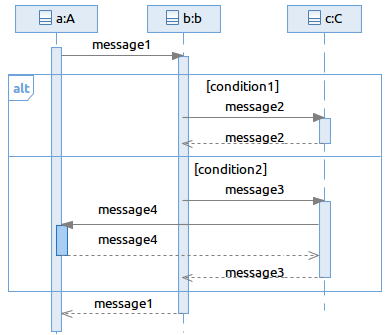
\includegraphics[width=0.5\linewidth,keepaspectratio=true]{./Figure4_new.png}
\caption{Sequence Diagram example}
\label{fig:counterExample}
\end{figure}
% \vspace{-10 pt}
Even if we assume that the scenario is executed by a single OS process, treating 
each object as a sequential process is problematic. In the example, after invocation of \emph{message1}, object \emph{a}
needs to know the choice that object \emph{b} has made (modeled with the \emph{alt} fragment), while this choice is based on local conditions that only \emph{b} is aware of. Therefore, \emph{a}
cannot know whether its method \emph{message4} will be invoked by object \emph{c}, before a return from \emph{message1} is received on the same lifeline.
Consequently, a single process representation of the lifeline \emph{a} should not control the reception of \emph{message4} and execution of the associated behavior.
Some approaches attempt to deal with this by making all involved processes aware of each others' local decisions, but this quickly becomes cumbersome and prone to errors, given
how complex UML 2.x SDs can be made by nesting combined fragments.

We wish to preserve the OO paradigm in the transformation to a formal model. In this paradigm, unless an object is active, 
it does not control the invocation of its methods; it only responds by executing the associated behavior. 
An OS process is then essentially a chain of method invocations on objects. To achieve this, we associate an mCRL2 process \emph{description} with each class method.
A description (be it actual program code or a UML model) of a class method should not differ across objects that are instances of that class. 
Of course, at runtime objects execute only one of the multiple possible traces captured by that description, based on variable values. 
In our methodology, each such mCRL2 process \emph{instance} carries data parameters that encode the class, object, and OS process instance to which the
exhibited method behavior belongs at runtime. As an important consequence of this choice, \emph{we preserve information on objects, classes and method calls in the mCRL2 model}, which
makes it easy to reverse model-checking traces back into the UML domain.
\vspace{-8 pt}
\subsection{The Approach}
\vspace{-6 pt}
Figure~\ref{fig:approach} gives a general overview of our approach and implemented toolset. 
Both the source (UML) and the target (mCRL2) models adhere to their respective metamodels.
% % \vspace{-10 pt}
\begin{figure}
\centering
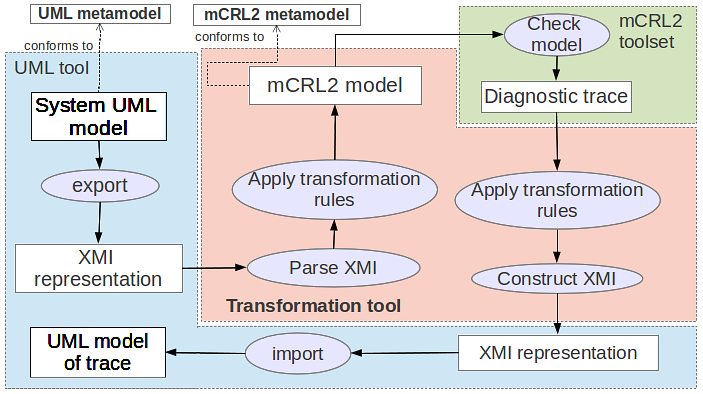
\includegraphics[width=0.8\linewidth,keepaspectratio=true]{./Approach.png}
\caption{Automated verification of UML models}
\label{fig:approach}
\end{figure}
% \vspace{-10 pt}
Although any mature UML modeling tool with XMI export/import capabilities can be used, we chose IBM's Rational environment
because of the excellent support for SDs and consistency preservation across multiple views of the same model.
For parsing and manipulation of the XMI representations we use Eclipse's MDT-UML2 plugin, which implements the UML 2.x metamodel.
The transformation rules define how to incrementally generate a model that conforms to a
particular metamodel, from a model that conforms to another metamodel.

To achieve the basic idea of mapping each method along a lifeline into an mCRL2 process description, we process the ordered events along every
lifeline individually, thus decomposing the lifeline into individual \emph{ExecutionSpecifications}. 
We take into account both synchronous and asynchronous messages, 
so there are essentially 6 different types of message events (shown in Fig.~\ref{fig:exampleProcesses}) that we consider: 
(1) \emph{SendEvent}\textunderscore\emph{synchCall}; (2) \emph{SendEvent}\textunderscore\emph{reply}; (3) \emph{ReceiveEvent}\textunderscore\emph{synchCall}; 
(4) \emph{ReceiveEvent}\textunderscore\emph{reply};
(5) \emph{ReceiveEvent}\textunderscore\emph{asynchCall}; and (6) \emph{SendEvent}\textunderscore\emph{asynchCall}.
\vspace{-10 pt}
\begin{figure}
\centering
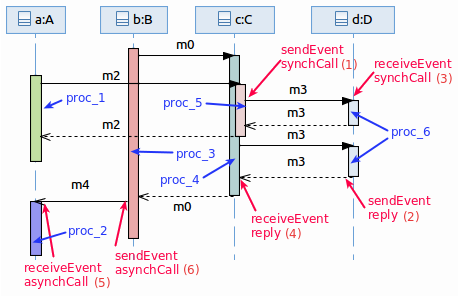
\includegraphics[width=0.65\linewidth,keepaspectratio=true]{./Figure6.png}
\caption{Identifying event types along lifelines}
\label{fig:exampleProcesses}
\end{figure}
\vspace{-10 pt}
In UML metamodel terms, each of these events correspond to \emph{MessageOccurrenceSpecifications}, and refer to the ends of each \emph{Message}.
Readers familiar with the UML metamodel are referred to Fig.~\ref{fig:SDMetamodel}
  for a simplified class diagram of the Interactions metamodel,
  though the transformation process in the sequel can be understood
  without it.
An \emph{Interaction} (a Sequence Diagram)
essentially encloses \emph{Messages}, \emph{Lifelines} and an ordered list of \emph{InteractionFragments}.
Each \emph{Message} is accompanied by a pair of \emph{MessageOccurrenceSpecifications}, and has a reference to
the lifeline from which the message is sent and to which that message is received. 
Both \emph{MessageOccurrenceSpecifications} and \emph{CombinedFragments} (omitted from the figure for clarity) 
are specializations of \emph{InteractionFragment}.
We exploit these relationships in our algorithm for matching and transforming into an mCRL2 model.
\vspace{-6 pt}
\begin{figure}
\centering
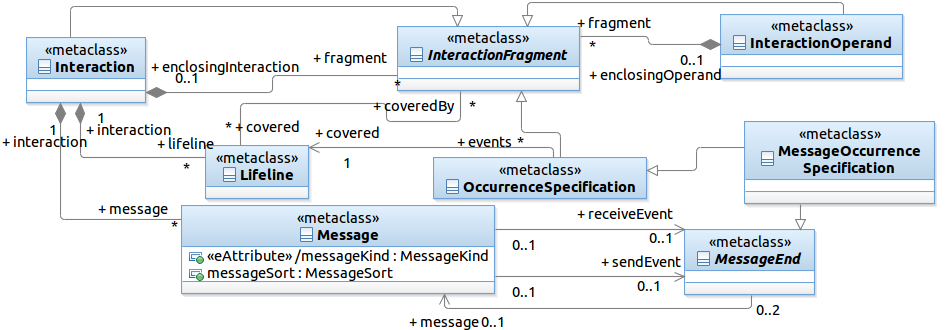
\includegraphics[width=1.05\linewidth,keepaspectratio=true]{./Profile_SDMetamodel1.png}
\caption{Selected elements of the Interactions metamodel}
\label{fig:SDMetamodel}
\end{figure}
\vspace{-6 pt}

% The main algorithm steps are given in continuation.
All fragments of an \emph{Interaction} are processed sequentially, and depending on their type,
different mapping rules are applied. In case of \emph{MessageOccurrenceSpecifications}, each event type is treated separately.
In case of a \emph{CombinedFragment}, each \emph{InteractionOperand}'s nested fragments are treated by applying the same procedure recursively.
$\\$   
\hrule

\alglanguage{pseudocode}
% \begin{algorithm}[h]
% \caption{Part 1}
\begin{algorithmic}[1]
\Procedure{processFragments}{$fragments \gets interaction.getFragments()$}
\For{\textbf{each} $fragment$ in $fragments$}
% $quality\ge 9$
\If{$fragment.type = MessageOccurrenceSpecification$}
  \State $message \gets fragment.getMessage()$
  \State $arguments \gets message.getArguments()$
  \State $event \gets fragment.getEvent()$
  \State $objName,className \gets fragment.getCovered.getObjectAndClass()$
  \State $theReadyStack \gets readyProcessesPerLifeline.get(objName)$
  \State $theBusyStack \gets busyProcessesPerLifeline.get(objName)$
      \algstore{bkbreak}
\end{algorithmic}
% \end{algorithm}
\hrule
$\\$
Two in-memory stacks are kept for the currently ``ready'' and the ``busy'' methods on each lifeline, for cases of overlapping invocations.
Busy methods are waiting (blocked) for a reply from another method execution that they have invoked, while ready processes are active, but not blocked.
The message, arguments, class, and object corresponding to the handling event are retrieved.
$\\$
\hrule
% \begin{algorithm}
\alglanguage{pseudocode}
% \begin{algorithm}[h]
% \caption{Part 1}

\begin{algorithmic}[1]
\algrestore{bkbreak}
  \Switch{$event$}
    \Case{$SendEvent \_ synchCall:$} \Comment{ Case (1)}
      \State $mcrl2Process \gets theReadyStack.pop()$
      \If{$insideInteractionOperand \And firstEvent$}
	\State $operator \gets getCombinedFragmentOperand()$
	\State $guard \gets getCombinedFragmentOperandGuard()$
	\If{$operator="alt"$}
	  \State $mcrl2Process.addAltFragment(guard)$
% 	  \ElsIf{$operator="opt"$}
% 	   \State $mcrl2Process.addOptFragment(guard)$
% 	   \ElsIf{$operator="break"$}
% 	   \State $mcrl2Process.addBreakFragment(guard)$
	    \State 
	      [...]
	      \ElsIf{$operator="par"$}
	   \State $mcrl2Process.addParFragment(guard)$
	  \ElsIf{$operator="loop"$}
	    \State $loopProcess \gets new LoopProcess()$
	    \State $mcrl2Process.addCallToLoopProcess(loopProcess)$
	    \State $theReadyStack.push(mcrl2Process)$
	    \State $loopProcess.addCondition(guard)$					
	\EndIf
	  \EndIf
	\State $mcrl2Process.addInvocation($
	      \State $"synch \_ call \_ send(id,className,objName,message,arguments)")$
	\State $theBusyStack.push(theProcess)$				
    \EndCase
    \algstore{bkbreak}
\end{algorithmic}
% \end{algorithm}
% \hspace{\fill}\rule{1.0\linewidth}{.3pt}\hspace{\fill}%
 
\hrule
$\\$  
The above pseudocode handles the case of \emph{SendEvent\_synchCall} observed on a lifeline. For invocation to be possible,
the object representing that lifeline must already be active in some method, at the same time \textbf{not} being blocked and awaiting for a return from a method call. 
We obtain that ``ready'' method (or mCRL2 \emph{process}) from a stack, on line 12. 
In addition, this is the only valid UML case where it is possible
for a \emph{SendEvent\_synchCall} to be the first event inside a \emph{CombinedFragment}. The different fragment types 
are handled by associating a corresponding mCRL2 structure in the mCRL2 process (lines 14-27). The details of how each type of fragment is mapped
to an mCRL2 structure will be explained after the algorithm walk-through, where also invocations (line 28) added to each process will be discussed.
$\\$  
\hrule
\begin{algorithmic}[1]
\algrestore{bkbreak}
    \Case{$SendEvent \_ reply:$} \Comment{ Case (2)}
      \State $mcrl2Process \gets theReadyStack.pop()$
      \State $mcrl2Process.setProcessed()$
      \State $mcrl2Process.addInvocation("$
        \State $synch \_ reply \_ send(id,className,objName,message,arguments)")$
      \EndCase  
      \algstore{bkbreak}
\end{algorithmic}

\hrule
$\\$   
Once a method sends a reply (\emph{SendEvent\_reply}), that mCRL2 process description is finished. The process is removed from the appropriate ``ready'' stack, 
as it no longer exhibits behavior after this point.
$\\$  
\hrule

\begin{algorithmic}[1]
\algrestore{bkbreak}
    \Case{$ReceiveEvent \_ synchCall:$} \Comment{ Case (3)}
	\State $findProcess \gets findProcess(className, message)$
		\If{$findProcess=null$}	
		  \State $findProcess \gets new Process(className, message)$
		 \EndIf
		 \If{$ \neg findProcess.isProcessed$}
		    \State $theReadyStack.push(findProcess)$
		    \State $findProcess.addInvocation($
		     \State $"synch \_ call \_ receive(id,className,objName,message,arguments)")$
		  \EndIf
	\EndCase	
	      \algstore{bkbreak}
\end{algorithmic}
\hrule
$\\$   
Reception of a synchronous call on a lifeline indicates method invocation. Unless the mCRL2 process corresponding to this method has already been
fully constructed, a new one is created, and pushed to the ``ready'' stack.
% $\\$  
% \hrule
% \begin{algorithmic}[1]
% \algrestore{bkbreak}
% 	 \Case{$ReceiveEvent \_ reply:$} \Comment{ Case (4)}
% 	  \State $findProcess \gets theBusyStack.pop()$
% 	  \State $theReadyStack.push(findProcess)$
% 	  \State $findProcess.$
% 	  \State $addInvocation($
% 	  \State $"synch\_ reply\_ receive(id,className,objName,message,arguments)")$
% 	\EndCase		
% \algstore{bkbreak}
% \end{algorithmic}
% 
% \hrule
% $\\$  
\vspace{-8 pt}
\begin{figure}
\centering
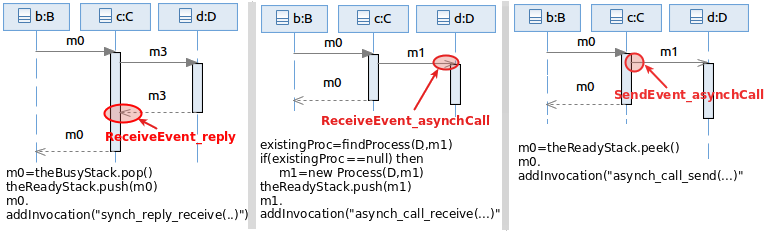
\includegraphics[width=1.0\linewidth,keepaspectratio=true]{./aman_full.png}
\caption{Handling Case 4(left), Case 5(middle) and Case 6(right)}
\label{fig:Algo}
\end{figure}
\vspace{-8 pt}

To get an intuition on how the algorithm proceeds, we treat Cases 4, 5, and 6 along with a graphical notation (Fig.~\ref{fig:Algo}), rather than an algorithmic exposition. 
Upon reception of a reply from a method (Case (4)), the one initiating it is no longer
blocked, so the corresponding mCRL2 process is removed from the ``busy'' stack
and added to the ``ready'' one.
Handling of Case (5) is analogous to Case (3), except that a different
kind of invocation is added to the mCRL2 process.
Finally, handling Case (6) is also analogous to Case (1), with the important difference being that the active method invoking this asynchronous call on another object
will not be blocked after the call. This is why the process is not removed from the ``ready'' stack nor pushed to the busy one.
$\\$  
\hrule
\begin{algorithmic}[1]
\algrestore{bkbreak}
\EndSwitch
  \ElsIf{$fragment.type = CombinedFragment$}
  \State $\textbf{getOperandsForCombinedFragment}(fragment)$
 \EndIf
\EndFor
\EndProcedure
\end{algorithmic}
\hrule
 $\\$   
\hrule
\alglanguage{pseudocode}
\begin{algorithmic}[1]
\Procedure{getOperandsForCombinedFragment}{$fragment$}
\State $operands \gets fragment.getOperands()$
% \For{$\textbf{each} operand in operands$}
\For{\textbf{each} $operand$ in $operands$}
  \State $processFragments(operand.getFragments())$ \Comment{handle recursively}
\EndFor	
\EndProcedure
\end{algorithmic}
\hrule
$\\$  
All operands that belong to a \emph{CombinedFragment} are processed in turn, recursively handling all fragments (possibly also nested \emph{CombinedFragments}) contained in them, by
calling \emph{processFragments} again. This concludes the basic algorithm for transformation of SDs of arbitrary complexity into mCRL2 process descriptions.
When the algorithm is applied to the example in Fig.~\ref{fig:exampleProcesses} it should result in 6 different process definitions.
The data that messages convey, and which takes part in decisions, are owned by the objects representing the lifelines.
This data is maintained by introducing a recursive ``memory'' process for each object within the mCRL2 specification, which carries all data values as parameters
\cite{remenska:using}.
% For details on how this is achieved, the reader can refer to \cite{remenska:using}.
Most of the primitive data types used have a direct mapping into mCRL2 types. 
Strings are handled using mCRL2's abstract data type capabilities.
Due to space limitations we will not explain the transformation rules for activity diagrams, 
although they are rather simple. We will demonstrate them on an example instead.

The different invocation types added to the mCRL2 processes in the course of the transformation are mCRL2 actions.
They carry all parameters necessary for exchange of data between processes, and are used for synchronizing the processes
on the corresponding send/receive events. The actions \emph{synch\_call\_send} and \emph{synch\_call\_receive} represent
two ends of a synchronous message exchanged between two processes. Similarly, \emph{synch\_reply\_send} 
and \emph{synch\_reply\_receive} correspond to a reply message, while \emph{asynch\_call\_send} and \emph{asynch\_call\_receive} 
represent an asynchronous call. By applying the mCRL2 communication ($\Gamma$) and allow ($\Delta$) operator in the following manner:
\vspace{-10 pt}
\begin{center}
$ \Delta_{\{synch\_call,\ synch\_reply, } $
  $    _{asynch\_call\}} $
  
$ \Gamma_{\{synch\_call\_send|
   synch\_call\_receive} $
  $  _{\rightarrow synch\_call, } $
%  $ \\ $
  $ _{synch\_reply\_send|synch\_reply\_receive} $
  $  _{\rightarrow synch\_reply,} $
%    $\\$
 $ _{asynch\_call\_send|asynch\_call\_receive} $
  $  _{\rightarrow asynch\_call\}} $
%$ \\ $
%$ \\ $
\end{center}
% \vspace{-2 pt}
communication is enforced between processes as a result of the multi-action synchronization at the corresponding events. 

Figure~\ref{fig:application1} demonstrates the transformation rules on a simple example. 
Classes, objects, method names and string values
are represented by enumerated data types (\textbf{struct}). 
Replies are distinguished from their respective method calls, as they may also carry
parameters. The mCRL2 summation (\textbf{sum)} operator is used for binding parameter identifiers to actual values when two processes communicate. 
This example illustrates how the \emph{alt} fragment is translated into the mCRL2 conditional operator. To avoid deadlocks, and permit the process
to continue in case none of the guards evaluates to true, the \textbf{internal} (${\tau}$) step is added as a last choice. The translation
of the \textit{opt} and \textit{break} fragments uses the conditional operator in a very similar manner. In a \textit{par} fragment,
all communication inside each operand is set to run in parallel with the  ``${||}$'' mCRL2 operator.
The \textit{loop} fragment has a special treatment. It is translated into a recursive process referenced by the mCRL2 process representing
the method active at the moment of entering the loop.
% \vspace{-8 pt}
\begin{figure*}[tp!]
  \centering
  \subfloat[Application of the SD transformation rules]{\label{fig:application1}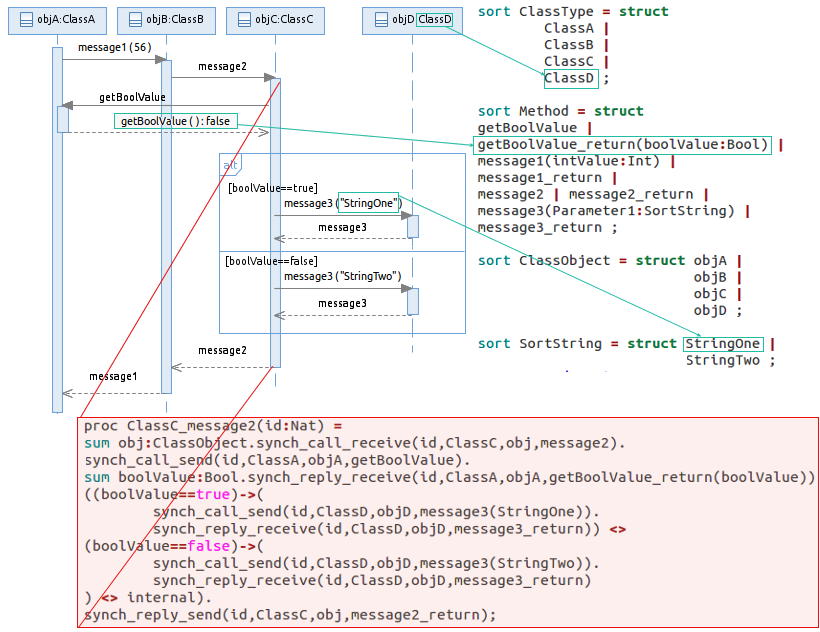
\includegraphics[width=1.0\linewidth]{./yea1.png}}    
%   \vfill
%   \hfill
  \vspace{28 pt}
  \subfloat[Application of AD transformation rules for system-level concurrency setup]{\label{fig:finally}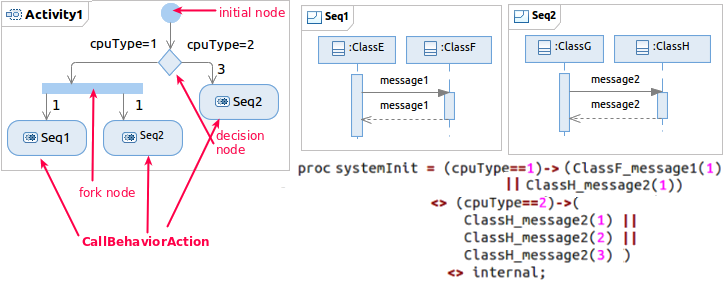
\includegraphics[width =1.0\linewidth]{./Figure9_new.png}}
  \caption{Transformation methodology by example}
%   \label{fig:finally}
\vspace{-8 pt}
\end{figure*}

Finally, Fig.~\ref{fig:finally} shows how a simple system-level concurrency can be expressed in an AD, and how it is translated into an mCRL2 specification.
ADs consist of \emph{Actions} and \emph{Control Nodes} connected by \emph{Activity Edges}, with each diagram having one \emph{Initial Node}. The 
control nodes have their intuitive meaning as in traditional flow charts, namely to depict concurrent flows (\emph{Fork}), and decision points (\emph{Decision}).
While there are various action types, we are primarily interested in the \emph{CallBehaviorAction}, which invokes a referenced behavior directly. Since
SDs are classified as behavior, we use this action type to provide the link between SDs and the concurrent system setup described in an AD. In the given example,
depending on the condition,
three concurrent OS process instances are started with the \emph{Seq2} SD, or alternatively one instance of \emph{Seq1} and \emph{Seq2} in parallel. 
The \textit{id:Nat} parameter that each mCRL2 process carries is used to bind it to an OS process in the system setup. It is also possible to
add \emph{Activity Final Node} for systems where execution terminates, by design.
%
% \vspace{-6 pt}
% \begin{figure}
% \centering
% 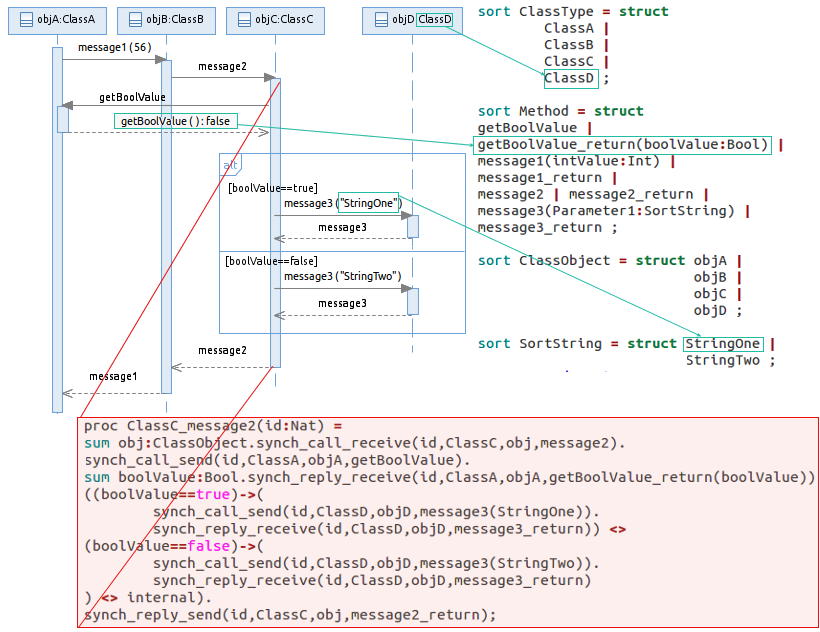
\includegraphics[width=1.0\linewidth,keepaspectratio=true]{./yea1.png}
% \caption{Application of the transformation rules on an example}
% \label{fig:application1}
% \end{figure}
% % \vspace{-8 pt}
% 
% \begin{figure}
% \centering
% 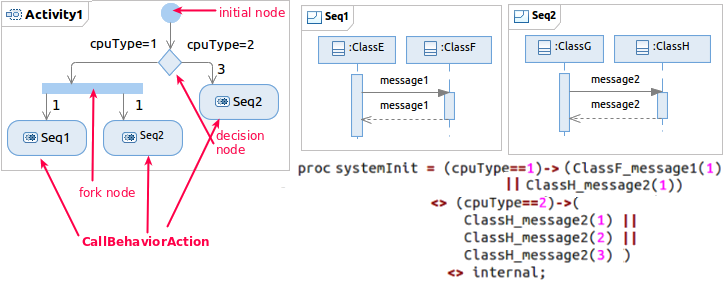
\includegraphics[width=0.97\linewidth,keepaspectratio=true]{./Figure9_new.png}
% \caption{Application of transformation rules for system-level concurrency setup}
% \label{fig:finally}
% \end{figure}
\vspace{-6 pt}
\section{Case Study:DIRAC’s Executor Framework}
\label{sec:Application}
\vspace{-6 pt}
DIRAC \cite{DIRAC_CommGridSolution} is the grid framework used to support production activities of the LHCb experiment at CERN.
Jobs submitted via its interface undergo several processing steps between the moment they are submitted to the grid, 
to the point when their execution on the grid actualizes. 
\begin{figure}
\centering
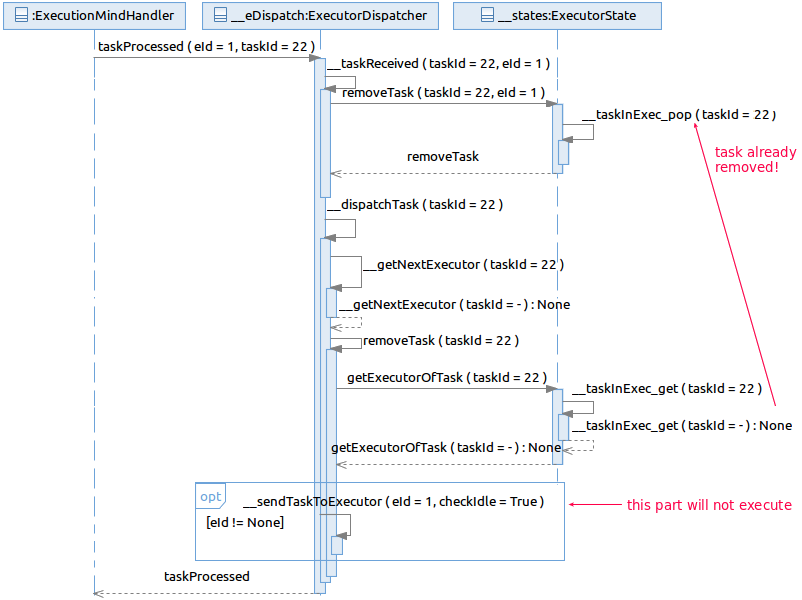
\includegraphics[width=1.0\linewidth,keepaspectratio=true]{./NoProgress2.png}
\caption{SD trace showing a case of no-progress of tasks scheduling}
\label{fig:noProgress}
\end{figure}
The crucial Workload Management components responsible for orchestrating this process are the \emph{ExecutorDispatcher} and 
the \emph{Executors}. Executors process any task sent to them by the ExecutorDispatcher, each one being responsible for a different step in the handling of tasks
(such as resolving the input data for a job).
The ExecutorDispatcher takes care of persisting the state of the tasks and distributing them amongst all the Executors, based on the
requirements of each task. It maintains a queue of tasks waiting to be processed, and other internal data structures to keep track
of the distribution of tasks among the Executors.

We used our toolset to generate an mCRL2 model based on the provided sequence diagrams of the Executor Framework. Using the mCRL2
toolset, we discovered a problematic behavior in the ExecutorDispatcher component, which results in no further progress of
submitted tasks. Such behavior is shown in Fig.~\ref{fig:noProgress}, obtained by transforming the mCRL2 trace into an SD, using
our toolset. 
The original trace is much longer (and available along with the model 
at \cite{repo:remenska}), here we only present the most important part for understanding the cause. 
Whenever a task has been processed by some of 
the Executors, the ExecutorDispatcher is notified (\emph{taskProcessed(eId,taskId)}), and this removes it from its internal list 
of processing tasks. To further dispatch the task to another Executor, this task is removed from the ExecutorDispatcher's memory of processing tasks,
followed by retrieval of the next responsible Executor. In case it was actually processed by the last Executor in the chain, the
 dispatcher attempts to retrieve its last Executor (\emph{getExecutorOfTask(taskId))}, so that more tasks can be dispatched by 
this (now free) Executor. However, this information
is already removed, as can be seen from the figure. As a result, the \emph{opt} fragment (shown only for clarity, not generated by the toolset)
will not be executed, and no further tasks waiting for this Executor will be dispatched. This was confirmed to occur in the real system, but
the cause could not be identified by testing.
\vspace{-10 pt}
% \vspace{-26 pt}
\section{Conclusions and Future Work}
\label{sec:Conclusions}
\vspace{-8 pt}
We have presented an automated transformation methodology for verification of UML models, based on sequence and 
activity diagrams, preserving the object-oriented view of the system in the transformation. 
Both the input and the output of our implemented toolchain are expressed in UML, so engineers
do not have to leave the UML environment, nor have a background in process algebra and model checking. 
We have further
applied our toolset to a use case from the domain of distributed object-oriented software, in particular to a component
of the DIRAC grid system used by the LHCb experiment at CERN, and discovered a logical flaw leading to no-progress.

Although the mCRL2 toolset automatically discovers deadlocks, model checking for application-specific properties 
requires the use of temporal logic on the generated model.
Part of the future work is expressing modal $\mu$-calculus formulas as sequence diagrams of accept/reject scenarios: 
behaviors that the designer wants to either confirm or avoid in the model. This can be easily achieved, given that
$\mu$-calculus formulas are action-based, and actions correspond to message exchanges in our transformation methodology.
Furthermore, we plan to explore the limitations of this approach, given that process proliferation is likely to happen
in larger systems. In our case study, we have as many as 50 processes, and already generating the entire state space can be problematic
at this scale, given that the generated model is over 2000 lines of model code.

Besides discovering behavioral problems, automating performance analysis is on our road-map as well.
UML provides extension mechanisms called \emph{Profiles} which allow annotating models with quantitative information,
such as expected execution time, resource usage, number of requests, etc. 
These quantities permit assessing the system’s efficiency and reliability. Our approach can be easily extended
in this direction, by taking into account not only message occurrences, but also annotated execution specifications
within SDs. We can use the same target formalism for enhancing the models with such quantitative information.
The CADP toolset~\cite{GaravelLMS11} for analysis of stochastic models is well integrated with mCRL2 for this
purpose.

\vspace{-10 pt}
\bibliographystyle{splncs} 
\bibliography{NASALibrary}

\end{document}
